\documentclass[11pt]{beamer}

\usepackage[utf8]{inputenc} 
\usepackage[T1]{fontenc}
\usepackage{lmodern}
\usepackage{graphicx}
\usepackage[french]{babel}
\usepackage{listings}
\usepackage{eurosym}
\usepackage{verbatim}
\usepackage{colortbl}

\setbeamertemplate{blocks}[rounded][shadow=true]
\expandafter\def\expandafter\insertshorttitle\expandafter{%
    \insertshorttitle\hfill\insertframenumber\,/\,\inserttotalframenumber}

% \onehalfspacing

% Espacement des lignes
%\linespread{1.2}

% Theme
\usepackage{animate}
\usetheme{Warsaw}                                % un theme voir .../beamer/theme/
\usecolortheme{orchid}
\usecolortheme{whale}


% Numéro diapo en bas
%\setbeamertemplate{footline}[frame number]

\title[Equipe segment SOL : Chef de PROJET]{Projet DRONE}
\subtitle{Gestion de L'OS Embarqué et de l'environnement Graphique}
\institute{ Ecole Supérieure des Technologies Electronique Informatique Infographie  }
\author{Pierre-jean \textsc{TEXIER}}
\date{13 Février 2014}
 

\hypersetup{% Modifiez la valeur des champs suivants
	pdfauthor   = {Texier Pierre-jean},%
	pdftitle    = {Présentation PROJET 2013-2014},%
	pdfsubject  = {Gestion de l'OS Embarqué et gestion de l'environnement Graphique},%
	pdfkeywords = {Mots clés},%
	pdfcreator  = {PDFLaTeX},%
	pdfproducer = {PDFLaTeX},%
}


\begin{document}
	% Diapositive
	\begin{frame}
	  \maketitle
		\begin{figure}
			\begin{center}
				\includegraphics[width=2cm]{common/estei.png}\\
				\includegraphics[width=1cm]{common/cc.png}
			\end{center}
		\end{figure}
	\end{frame}
		
	\begin{frame}
		\frametitle{Sommaire}
		%\framesubtitle{}
		\begin{columns}[t]
		\begin{column}{5cm}
		\tableofcontents[sections={1-4},hideallsubsections]
		\end{column}
		\begin{column}{5cm}
		\tableofcontents[sections={5-10},hideallsubsections]
		\end{column}
		\end{columns}
	 \end{frame}
	
	%%%%%%%%%%%%%%%%%%%%%%%%%%%%%%%
	
 	\section{Présentation du Projet}
	\begin{frame}{Présentation du Projet}
	\begin{center}
	
	\includegraphics[width=2cm]{common/estei.png}\\
	Projet de FIN d'étude \\
	``Contexte Industriel'' durant 6 mois\\
	PROJET Drone \textbf{\textsc{Next GEN}}   \\     
	2 Composants => 2 Equipes  
	\begin{center}
	\includegraphics[width=3cm]{common/drone.png}
	\end{center}
	\end{center}
	\end{frame}
	
	%%%%%%%%%%%%%%%%%%%%%%%%%%%%%%%
	
	\section{Segment SOL}
	\begin{frame}{Présentation du Segment SOL}
		\begin{itemize}
		    \item Présentation : station constituée d'une carte mère\\
		    \begin{center}
		    \includegraphics[width=2cm]{common/segment.png}\\
		    \end{center}
		    \pause
		    \item L'équipe (OBS : \textbf{O}rganization \textbf{B}reakdown \textbf{S}tructure)\\
		    \pause
		    \begin{center}
		    \includegraphics[width=7cm]{common/OBS.png}
		    \end{center}
		\end{itemize}
	\end{frame}
	
	%%%%%%%%%%%%%%%%%%%%%%%%%%%%%%%
	
	
	\subsection{Phase Programme}
	\begin{frame}{Expression des Besoins}
	\underline{Besoins Exprimés par le Client} :
	\newline
	\begin{itemize}
	 \item Affichage
	  \item Ergonomie
	   \item Vidéo
	    \item Communication
	    \item Gamme de Température
	    \begin{itemize}   
	    \item Commerciale : 0\textdegree C à  70\textdegree C
	    \item Industrielle :  -45\textdegree C à  85\textdegree C
	    \end{itemize}
	\end{itemize}
	\end{frame}
	
	
	%%%%%%%%%%%%%%%%%%%%%%%%%%%%%%%%%%%%%%ù
	
	\subsection{Analyse Fonctionnelle}
	\begin{frame}{Diagramme Fonctionnel de Degré 1}
	\begin{center}
		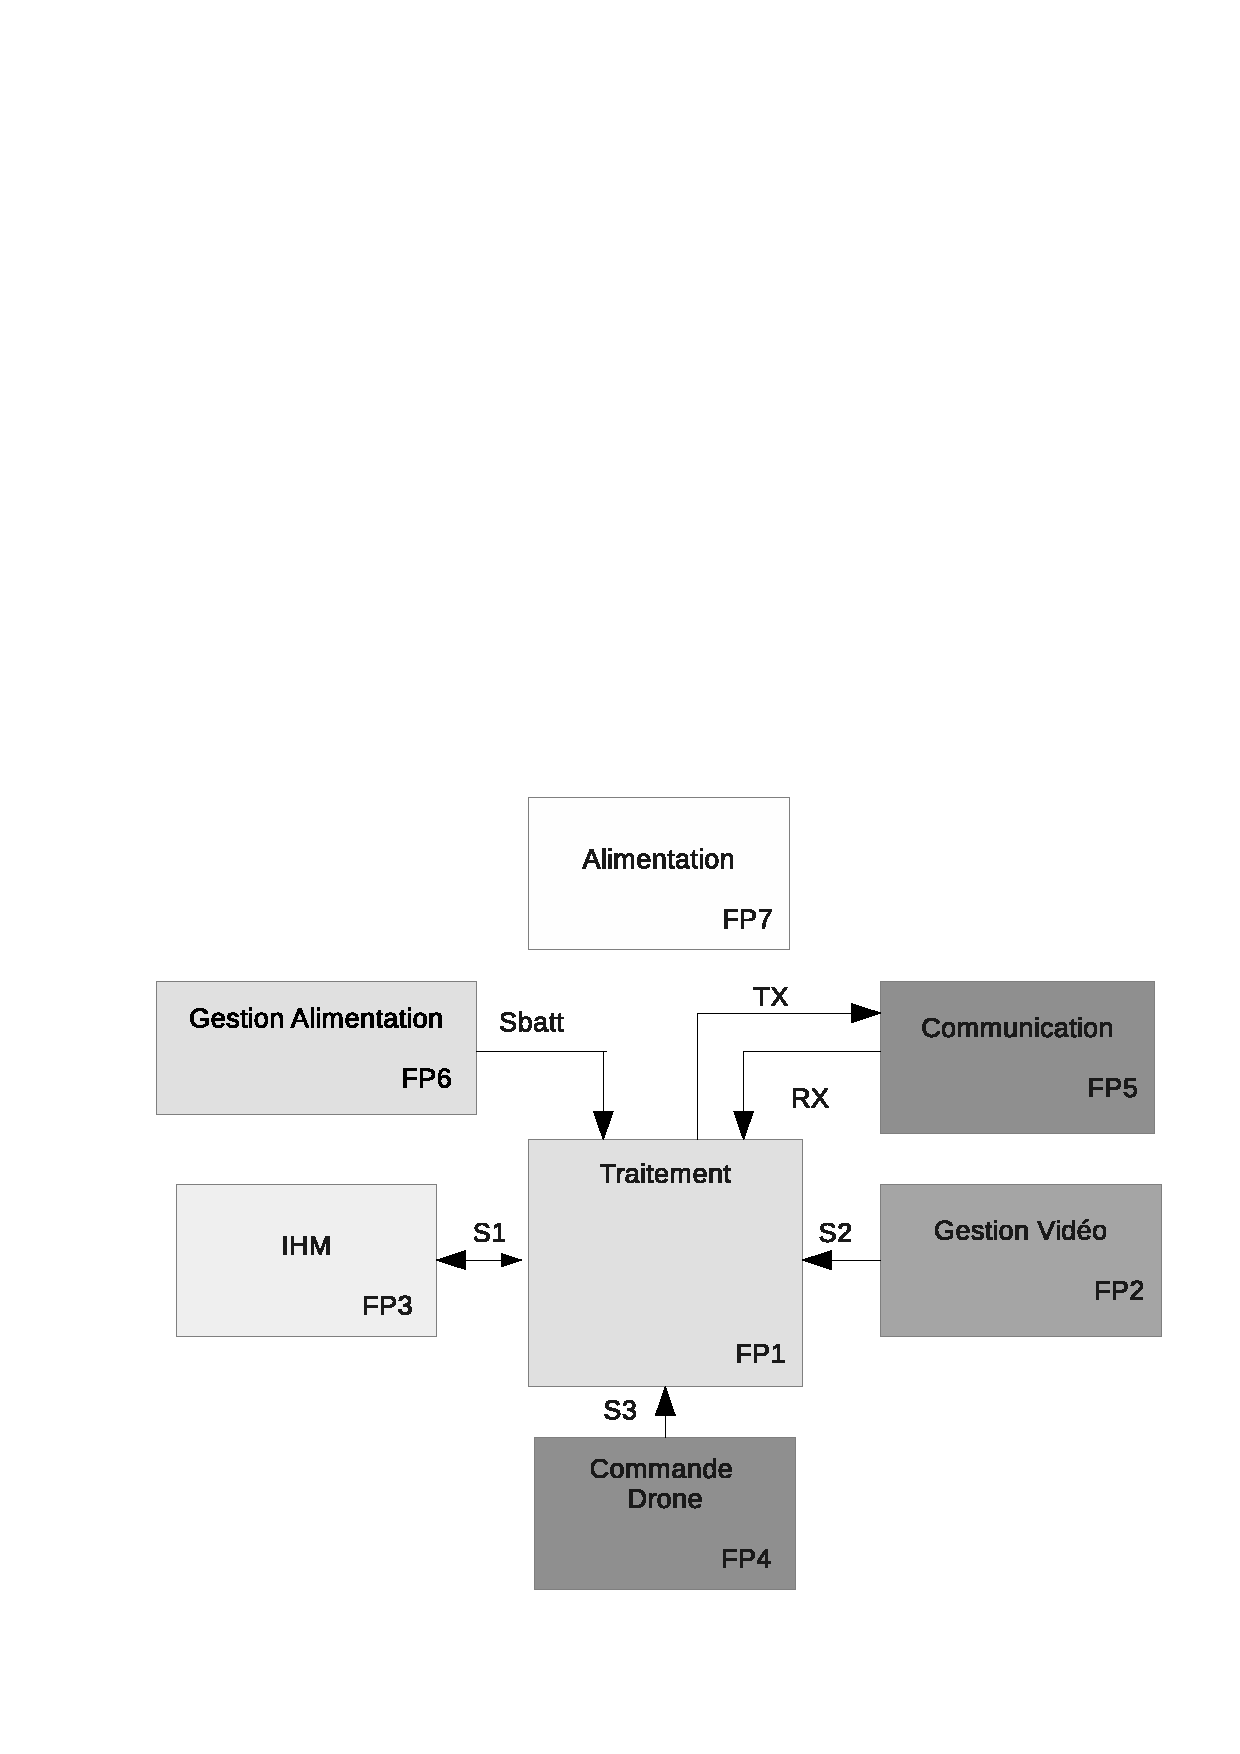
\includegraphics[width=7cm]{common/fonc.png}
	\end{center}
	\end{frame}
	
	\subsection{Matrice de Compétence}
	\begin{frame}{Matrice de compétence Segment SOL}
		\begin{center}
			\includegraphics[width=10cm]{common/matrice.png}
		\end{center}
			\begin{block}{Remarques}
			
			    \centering Permet d'organiser au mieux les ressources
			  
			\end{block}
	\end{frame}
	
		%%%%%%%%%%%%%%%%%%%%%%%%%%%%%%%
	
	\subsection{Cahier des Charges}
	\begin{frame}
		\frametitle{Cahier des Charges Personnel}
		\framesubtitle{FP1 - FP6}
		\begin{center}
				\includegraphics[width=3cm]{common/cdcperso.png}	\\ 
		\end{center}
	\begin{block}{Tâches à réaliser}
		\begin{itemize}
			\item OS Linux embarqué Fonctionnel
			\item Préparation de l'environnement graphique (Qt, openCV, ...)
			\item Optimisation du temps de boot \textbf{hardware} et \textbf{subjectif}
			\item Gestion de l'énergie
		\end{itemize}
	\end{block}
	
	\end{frame}
	
	%%%%%%%%%%%%%%%%%%%%%%%%%%%%%%%
	
	%%%%%%%%%%%%%%%%%%%%%%%%%%%%%%%%%%%%%%ù
	
	\section{Gestion de Projet}
	
	\begin{frame}{Gestion de Projet}
		\begin{center}
			\includegraphics[width=5cm]{common/gestion.jpg}
		\end{center}
	\end{frame}
	
	\subsection{Cycle de vie Logiciel}
	\begin{frame}{Cycle de vie Logiciel}
		\begin{center}
			\includegraphics[width=10cm]{common/V.png}
		\end{center}
	\end{frame}
	\subsection{ROADMAP}
	\begin{frame}{ROADMAP : Segment SOL}
		\begin{center}
			\includegraphics[width=10cm]{common/roadmap.png}
		\end{center}
		\begin{block}{Remarques}
		\begin{itemize}
			\item 2 Jalons : Intégration
			\item Suivi du cycle de Vie Logiciel
		\end{itemize}
		\end{block}
	\end{frame}
	
	\subsection{Suivi des Dépenses}
	\begin{frame}{Suivi des dépenses : Segment SOL}
		\begin{center}
			\includegraphics[width=10cm]{common/depenses.png}
		\end{center}
		\begin{block}{Ce qu'il faut retenir}
		\begin{itemize}
			\item 750 Euros de Budget à l'instant t0
			\item Environ 450 Euros dépensés en fin de PROJET
		\end{itemize}
		\end{block}
	\end{frame}
	
	%%%%%%%%%%%%%%%%%%%%%%%%%%%%%%%
	
	\subsection{Diagramme de GANTT}
	\begin{frame}{Gantt Prévisionnel}
		\begin{center}
			\includegraphics[width=10cm]{common/Gantt.png}
		\end{center}
		\begin{block}{Remarques}
			\centering Les tâches du cahier des charges sont présentées ainsi que les relations entre elles
		\end{block}
	\end{frame}
	
	%%%%%%%%%%%%%%%%%%%%%%%%%%%%%%%
	
	\subsection{Outils}
	\subsubsection[]{Outils mis en place}
	\begin{frame}{Outils mis en place}
	Gestion de Version
	\begin{itemize}
	 \item GIT 
	      \begin{itemize}
	      \item \href{https://github.com/estei-master/segment_SOL}{\beamergotobutton{GITHUB Segment SOL}}
	      \end{itemize}
	 \end{itemize}
	 Gestion de Documentation
	 \begin{itemize}
	 \item Doxygen 
	      \begin{itemize}
	      \item \href{http://78.231.214.8/ihm2/html/}{\beamergotobutton{Doxygen Segment SOL}}
	      \end{itemize}
	  \end{itemize}
	  Gestion de Publication 
	  \begin{itemize}
	 \item Doku-Wiki 
	    \begin{itemize}
	    \item \href{http://78.231.214.8/dokuwiki/doku.php}{\beamergotobutton{Wiki Segment SOL}}
	    \end{itemize}
	\end{itemize}
	
	\end{frame}
	
%%%%%%%%%%%%%%%%%%%%%%%%%%%%%%%%%%%%%%%%
	
	\section{Droit}
	
	\begin{frame}{Droit}
	2 types de Licences utilisées pour le Projet
	\begin{itemize}
		\item GPLv3 \includegraphics[width=0.4cm]{common/gnu.png}	\\
		\href{http://www.tldrlegal.com/license/gnu-general-public-license-v3-(gpl-3)}{\beamergotobutton{Texte GPLv3}}
		
	\end{itemize}
	\begin{itemize}
		\item Creative Commons 	\includegraphics[width=1cm]{common/cc.png}\\
		\href{http://creativecommons.org/licenses/by-sa/4.0/}{\beamergotobutton{Texte Creative Commons}}

	\end{itemize}
	\begin{block}{A savoir}
			\begin{itemize}
			\item Développement avec des Outils Libres
			\item Améliore la \textbf{Maintenabilité}, \textbf{Portabilité} du développement
		\end{itemize}
		\end{block}
	
		\begin{block}{Quelques Outils}
			\begin{itemize}
			\item GIMP, GNU Linux, GNU plot, bootchart, \LaTeX, fbvis, ...
		\end{itemize}
		\end{block}
	\end{frame}
	%%%%%%%%
	
	\section{Réalisations}
	
	\begin{frame}{Réalisations}
		
			\begin{center}
			\includegraphics[width=2cm]{common/Settings.png}	
	\end{center}
		
	\end{frame}
	
	\subsection{Choix technologiques}
	\begin{frame}[label=choix]{Choix technologiques}
	\framesubtitle{Etude Materiel}
	\begin{itemize}
	\item System On Chip ?
	\begin{block}{Allwiner A20  \hyperlink{SoC}{\beamergotobutton{Synoptique}}\\}
	\begin{itemize} 
	
	  \item 2 processeurs : Dual Core ARM Cortex A7
	  \item 2 co-processeurs Graphique : GPU Mali 400MP2, ...
	\end{itemize}
	\end{block}
	
	\item Single Board Computer ?
	\begin{block}{OlinuXino A20 \hyperlink{SbC_2}{\beamergotobutton{Disponible sur le marché}}}
	\begin{itemize}  
	  \item 160 GPIO
	  \item Connecteur 40 Broches pour LCD, port Ethernet, ...\\
	\end{itemize}
	\end{block}
	\end{itemize}
	\end{frame}
	
	%%%%%%%%%%%%%%%%%%%%%%%%%%%%%%%%%%%%%%%%%%%%%%%%%%%
	
	\subsection{Environnement}
	\begin{frame}{Environnement ``Linux Embarqué''}
	\begin{center}
	\includegraphics[width=10cm]{common/arcg.png}	
	\end{center}
	\end{frame}
	
	
	\begin{frame}{Chaine de compilation croisée}
	\begin{block}{ Compilation Croisée ?}
	\centering Une chaîne de compilation croisée est un groupe d'outils permettant la compilation d'un programme d'une architecture processeur à une autre (x86 => ARM).
	\end{block}
	\pause
	\begin{columns}[b]
	\begin{column}{2cm}
	\begin{alertblock}{Mon Choix}
	\centering \includegraphics[width=1cm]{common/linaro.jpeg} %\textit{arm-*-gnueabihf-}
	\end{alertblock}
	\end{column}

	\begin{column}{8cm}
	\pause
	\begin{block}{Possibilitées}
	\centering Crosstool-ng, \includegraphics[width=1.5cm]{common/buildroot.png}, \includegraphics[width=0.8cm]{common/oe.png}
	\end{block}
	\end{column}
	\end{columns}
	\pause
	\begin{block}{Pourquoi HardFloat ?}
	\begin{itemize}
	 \item co-processeur : FPU neon-vfvp4
	\end{itemize}
	\end{block}

	\end{frame}
	
	\begin{frame}{Risques et Opportunités}
	\begin{center}
	  \includegraphics[width=10cm]{common/risques.png}\\
	\end{center}
	\end{frame}
	

	
	\subsection{Kernel in a Nutshell}
	\begin{frame}[label=Kernel]{Kernel in a Nutshell}
	Kernel ? \\ \hyperlink{Linux}{\beamergotobutton{Linux}}\\
	\pause
	Pourquoi Optimiser ?
	\pause
	 \begin{itemize}
	  \item Empreinte Mémoire
	  \pause
	  \item Besoins pour le Projet (V4L, Tactile, ...)
	 \end{itemize}
	  \pause
	  	\begin{columns}[t]
		\begin{column}{5cm}
		\begin{block}{Informations}
		\begin{itemize}
			\item Version 3.4.67
			\item Non mainline \\
			\href{https://github.com/linux-sunxi/linux-sunxi}{\beamergotobutton{Lien github}}
		\end{itemize}
		\end{block}
		\end{column}
		
		\begin{column}{5cm}
		\begin{block}{A savoir} 
		  \begin{itemize}
		    \item Plusieurs branches
		    \item 3.0 et 3.4.67 = stable
		    \item 3.10 = experimental
	\end{itemize}
	\end{block}
	\end{column}
	\end{columns}
	\end{frame}

	
	\begin{frame}{Configuration}

	 \begin{center}
	 \includegraphics[width=3cm]{common/tuxleg.png}\\
	 \end{center}
	 \begin{itemize}
		\item Interface : xconfig (\textbf{make ARCH=arm xconfig})
		\item Suppression : 
			\begin{itemize}
			    \item Options inutiles dans l'embarqué (\underline{ex} : Swap)
			    \item Options de Debug / Profilling (\underline{ex} : Ftrace)
			    \item Options Inutiles pour notre Projet (\underline{ex} : HDMI)
			 \end{itemize}
		 \end{itemize}
	 \begin{block}{Empreinte Mémoire}
	 \centering Début du Projet : \textbf{5.20 MB} --> Fin du Projet : \textbf{3.33 MB}
	 \end{block}	
	\end{frame}
	
	\begin{frame}{Implantation sur cible}
	\begin{itemize}
	 \item Système sur carte SD
	 \item u-boot, image noyau et script.bin sur la 1ère partition
	 \item rootFS sur la seconde partition
	\end{itemize}

	\centering \includegraphics[width=3cm]{common/SD.png}\\
	\end{frame}
	
	%%%%%%%%%%%%%%%%%%%%%%%%%%%%%%%
	
	\subsection{Graphique}
	\begin{frame}
	\begin{center}
	  Préparation de l'environnement \textbf{GRAPHIQUE}\\
	  \textit{``Fournir l'abstraction bas niveau avec le développement Logiciel'' }
	\end{center}
	\end{frame}
	
	\subsection{Qt embedded}
	\begin{frame}[label=pageQt]{Qt embedded  \includegraphics[width=0.3cm]{common/Qt.jpeg}}
	  \underline{Notre Contexte} : \hyperlink{Qt}{\beamergotobutton{Qt}}
	  \newline
	  \underline{Choix} : Affichage graphique \textbf{Framebuffer}
	  \newline
	  \newline
	  Qt embedded ? :
	  \begin{itemize}
			    \item Framework pour IHM et application embarqué
			    \item API Standard de Qt
			    \item Architecture Serveur/Client : QWS
			      \begin{center}
			       \includegraphics[width=4cm]{common/Qtembedded.png}\\
			      \end{center}
	   \end{itemize}
	  
	  
	  \end{frame}
	
	
	\begin{frame}[label=pageQt2]{Qt embedded  \includegraphics[width=0.3cm]{common/Qt.jpeg}}
	 \centering \underline{Ce qu'il nous faut} : ``qmake'' spécifique à notre architecture :
	\begin{block}{Etapes}
	\begin{enumerate}
			\item Choix et Cross-compilation de la librairie Tactile : tslib \hyperlink{tslib}{\beamergotobutton{tslib}}
			\item Modification du fichier \textbf{qmake.conf}
			\item Génération du Makefile spécifique aux besoins (./configure)
			\item Cross-compilation de Qt embedded 4.8.2 (make)
			\item Installation des binaires (make install)
			\item Portage des binaires générés sur cible
			\item Tests
	\end{enumerate}
	\end{block}	
	
	\end{frame}
	

	
	%%%%%%%%%%%%%%%%%%%%%%%%%%%%%%%
	
	\subsection{OpenCV embedded}
	\begin{frame}[label=pageopenCV]{OpenCV embedded}
	\begin{center}
	\includegraphics[width=1cm]{common/opencv.png}\\
	\end{center}
	Portage sur Architecture ARM
	\hyperlink{openCV}{\beamergotobutton{openCV}}\\
		\begin{block}{Etapes}
		\begin{enumerate}
			\item Choix des Modules openCV : Utilisation de Cmake
			\item Cross-compilation librairies/modules
			\item Portage des binaires générés sur cible
			\item Tests
	\end{enumerate}
	\end{block}	
	\end{frame}
	%%%%%%%%%%%%%%%%%%%%%%%%%%%%%%%
	
	\subsection{Optimisation démarrage}

	\begin{frame}{Optimisation du temps d'amorçage système}
	\begin{center}
	 \includegraphics[width=2cm]{common/boottime.png}
	\end{center}
	\end{frame}
	
	\subsubsection{Hardware}
	\begin{frame}[label=optimisation]{Hardware}
	U-boot
	\begin{itemize}
			\item Variable 'bootdelay'
	\end{itemize}
	Scripts de démarrage : \hyperlink{bootchart}{\beamergotobutton{bootchart}}\\
	\begin{itemize}
			\item Networking
			\item ssh
			\item exim4
			\item apache
	\end{itemize}
	\begin{block}{Temps de BOOT}
	 \centering Début du Projet : \textbf{1 minute} --> Fin du Projet : \textbf{33 secondes}
	 \end{block}	
	\end{frame}
	\subsubsection{Subjectif}
	\begin{frame}{Subjectif}
	Remplacement du Logo de démarrage : {\itshape \bfseries logo\string_linux\string_clut224.ppm}
	 \newline
	\begin{itemize}
	\item Logo de base 
		\begin{center}
		 \includegraphics[width=1cm]{common/logo_1.png}
		\end{center}
	\item Logo personnalisé : 640*480\footnote{modifier script.fex}
		\begin{center}
		 \includegraphics[width=3cm]{common/logo_2.png}
		\end{center}
	\end{itemize}
	\end{frame}
	
	\begin{frame}{PBIT}
	\framesubtitle{Power On Built in Test}
	\centering \textbf{Utilisation simpliste du Framebuffer pour la phase de ``PBIT''}
	 \newline
	 \begin{center}
	  \includegraphics[width=3cm]{common/PBIT1.png}
	 \includegraphics[width=3cm]{common/PBIT2.png}
	 \includegraphics[width=3cm]{common/PBIT3.png}
	 \newline
	 \includegraphics[width=3cm]{common/PBIT4.png}
	 \includegraphics[width=3cm]{common/PBIT5.png}
	\begin{block}

			\centering Cross-compilation de la librairie fbvis
	\end{block}
	 \end{center}


	\end{frame}
	%%%%%%%%%%%%%%%%%
	\subsection{Power Management}
	\begin{frame}[fragile]{Power Management}
	\begin{block}{Réalisé}
	\begin{itemize}
			\item Création d'un Crontab
			\item Test sur l'autonomie du Système
	\end{itemize}
	\end{block}
	
	\begin{center}
		\includegraphics[width=6cm]{common/power_management.png}
	\end{center}
	\end{frame}
	%%%%%%%%%%%%%%%%%%%
	\subsection{Optimisation du Système}
	\begin{frame}{Optimisation du Système}
	\framesubtitle{Réalisé}
	 \begin{itemize}
	 \item  Système de fichier Temporaire \\
	    	 \begin{itemize}
		    \item  \textit{tmpFS} (fichiers log)
		  \end{itemize}
	\item Autologin \\
	  	  \begin{itemize}
		    \item  \textit{agetty --autologin}
		  \end{itemize}
	\item Lancement Automatique de l'application : ihm\\
	\item UDEV \\
	  \begin{itemize}
		    \item iDVendor
		    \item iDProduct
	  \end{itemize}
	\end{itemize}
	\end{frame}
	
	%%%%%%%%%%%%%%%%%%%%%%%%%%%%%%%%%%%%%%%%%%%%%%%%%%%%%
	
	\begin{frame}{Optimisation du Système}
	\framesubtitle{Possible}
	 \begin{enumerate}
	 \pause
	 \item Accélération matérielle 
	\begin{center}
		\includegraphics[width=2cm]{common/opengles.png}
	\end{center}
	\pause
	 \item Gestion des Heuristiques : Variations dynamiques de fréquence processeur
	 \pause
	
	 \begin{itemize}
	 \item powersave
	 \pause
	 \item perfomance
	 \pause
	 \item ondemand
	 \pause
	 \item interactive, ...
	 
	 
	\end{itemize}
	 \end{enumerate}
	\end{frame}

	%%%%%%%%%%%%%%%%%%%%%%%%%%%%%%%%%%%%%%
	
	\section{Bilan de LOT}
	\subsection{LOT Segment SOL : Coûts}
	\begin{frame}{LOT Segment SOL : Coûts}
	Coût de Developpement   \includegraphics[width=0.5cm]{common/coins.png}\\
	\begin{center}
	\begin{tabular}{|c|c|}
			\hline
			\rowcolor{yellow}Nom / Prénom & Coût\\
			\hline
			TEXIER Pierre-jean  & 3300 \euro \\
			\hline
			PRADEAU Martin  & 2719 \euro \\
			%\hline
			POUCH Pierre  & 2640 \euro \\
			%\hline
			L'HUILLIER Guillaume  & 2640 \euro \\
			%\hline
			OUKRAT Rémi  & 19 669 \euro \\
			\hline
			\end{tabular}
			\end{center}
			
	Coût D'industrialisation \includegraphics[width=0.5cm]{common/industry.png} : 100 Pièces => 33905 \euro
	\end{frame}
	
	%%%%%%%%%%%%%%%%%%%%%%%%%%%%%%%%%%%%%%%%%%%%%%%%%%%%%
	
	\subsection{Conclusion}
	\begin{frame}{Conclusion}
	Lot Livrable
	\begin{center}
	 	\includegraphics[width=2cm]{common/deliverables.png} \\
	 	Intégration $\approx$ 80\%
	\end{center}
	GIT : \textbf{249 Commits}
	\begin{center}
	 	\includegraphics[width=6cm]{common/git.png} 
	\end{center}
	\end{frame}
	
	%%%%%%%%%%%%%%%%%%%%%%%%%%%%%%%%%%%%%%%%%%%%%%%%%%%%%
	
	\section{Conclusion}
	\subsection{Matrice de Validation}
	\begin{frame}{Matrice de Validation}

	\begin{center}
	\begin{tabular}{|p{3cm}|c|c|}
			\hline
			\rowcolor{yellow}Cahier des Charges & TV & Commentaires\\
			\hline
			 \centering Choix SoC / SbC & Levée de risque sur carte & \includegraphics[width=0.5cm]{common/ok.png} \\
			\hline
			 \centering Chaine de \par compilation croisée & Compilation ``hello world'' & \includegraphics[width=0.5cm]{common/ok.png} \\
			\hline
			 \centering OS Linux sur cible & Sur carte SD & \includegraphics[width=0.5cm]{common/ok.png} \\
			\hline
			 \centering Préparation graphique & Qt / OpenCV & \includegraphics[width=0.5cm]{common/ok.png} \\
			\hline
			 \centering Power Management & Via sysFS & \includegraphics[width=0.5cm]{common/ok.png} \\
				
			\hline
			\end{tabular}
	\end{center}
	\end{frame}

	\subsection{Conclusion}
	\begin{frame}{Conclusion}
	Compétences Acquises
		\begin{center}
		\begin{itemize}
			\item Portage d'application graphique sur \textit{Architecture ARM}
			\item Optimisation d'un système Linux
			\item Gestion d'un Projet de bout en bout : \textit{Chef de Projet}
		\end{itemize}
		\end{center}
	Bilan Personnel
		\begin{center}
		\begin{itemize}
			\item Mise en pratique de l'enseignement \includegraphics[width=1.5cm]{common/estei.png}
			\item Orientation en \textit{Linux Embarqué} confortée
			\item Atout pour le prochain stage
			\item Implication dans la communauté ``SUNXI''
		\end{itemize}
		\end{center}
	\end{frame}
	
	\subsection{Questions}
	\begin{frame}{FIN}	
	Tests de Validation
	\begin{enumerate}
	 \item Démarrage
	  \item Version du noyau
	    \item Démo Qt embedded
	\end{enumerate}

		\begin{center}
		  \includegraphics[width=2cm]{common/appli.png}
		\end{center}
	Questions 
		\begin{center}
		  \includegraphics[width=1.5cm]{common/dialog-question.png}
		\end{center}
	\end{frame}
	
%%%%%%%%%%%%%%%%%%%%%%%%%%%%%%%%%%%%%%%%%%%%%%%%%%%%%%%%%%%%%%%%%%%
	\begin{frame}[label=Linux]{Système Linux}
	 \begin{center}
		\includegraphics[width=8cm]{common/kernel.png}
	 \end{center}
	\hyperlink{Kernel}{\beamerreturnbutton{retour}}
	\end{frame}
	
	\begin{frame}[label=SoC]{Synoptique du System On Chip}
	 \begin{center}
		\includegraphics[width=7cm]{common/SoC.png}
	 \end{center}
	\hyperlink{choix}{\beamerreturnbutton{retour}}
	\end{frame}
	
	
	\begin{frame}[label=SbC_2]{Etude du Marché}
	 \begin{center}
		\includegraphics[width=2.5cm]{common/rpi.jpg}
		\includegraphics[width=2.5cm]{common/Panda.png}
		\includegraphics[width=2.5cm]{common/odroid.jpg}
		\includegraphics[width=2.5cm]{common/Cubieboard.jpeg}
	 \end{center}
	\hyperlink{choix}{\beamerreturnbutton{retour}}
	\end{frame}
	
	\begin{frame}[label=Qt]{Qt embedded}
	\begin{center}
			  \includegraphics[width=8cm]{common/Qt_arch.png}
		\end{center}
		\hyperlink{pageQt}{\beamerreturnbutton{retour}}
	\end{frame}
	
	\begin{frame}[label=tslib]{tslib}
	\begin{center}
			  \includegraphics[width=6cm]{common/tslib.png}
		\end{center}
		\hyperlink{pageQt2}{\beamerreturnbutton{retour}}
	\end{frame}
	
	\begin{frame}[label=openCV]{openCV}
			\begin{center}
			  \includegraphics[width=6cm]{common/v4l.png}
		\end{center}
		\hyperlink{pageopenCV}{\beamerreturnbutton{retour}}
	\end{frame}
	
	\begin{frame}[label=bootchart]{bootchart}
			\begin{center}
			  \includegraphics[width=4cm]{common/bootchart.png}
		\end{center}
		\hyperlink{optimisation}{\beamerreturnbutton{retour}}
	\end{frame}
%%%%%%%%%%%%%%%%%%%%%%%%%%%%%%%%%%%%%%%%%%%%%%%%%%%%%%%%%%%%%%%%%%%
\end{document}
